\subsubsection{Delete a Reservation}
			To accompany this diagram, read the Scenario \hyperref[sec:ReservationDeletionScenario]{S.11}.

				\begin{table}[htpb]
					\centering
					\label{tab:ReservationDeletionTable}
					\begin{tabularx}{\textwidth}{lp{9cm}}
						\hline
						\hline
							\textbf{Subject}
						& 
							\textbf{Description}\\
						\hline
							Actors	       &  Customer, myTaxiService Web Application, myTaxiService Server\\
						\hline
							Preconditions  &  Customer must be on the homepage and is already logged in.\\
						\hline
							Execution      &  1.~Customer taps on the "My Reservations" button.\\
										   &  2.~myTaxiService Mobile Application downloads the reservation list.\\
										   &  3.~myTaxiService Mobile Application shows the reservation list page.\\
										   &  4.~Customer selects the reservation to delete\\
										   &  5.~Customer deletes the reservation by pressing the "X" button.\\
										   &  6.~myTaxiService Mobile Application calls the server function to delete a reservation.\\
										   &  7.~myTaxiService Mobile Application shows a success notification.\\
						\hline
							Postconditions &  The Customer has deleted his reservation successfully.\\
						\hline
							Exceptions     &  1.~The Customer GPS is off.\\
							               &  2.~The Customer disconnects before the reservation.\\
									
						\hline
						\hline
					\end{tabularx}
				\end{table}
				
				\begin{figure}[H]
					\centering
					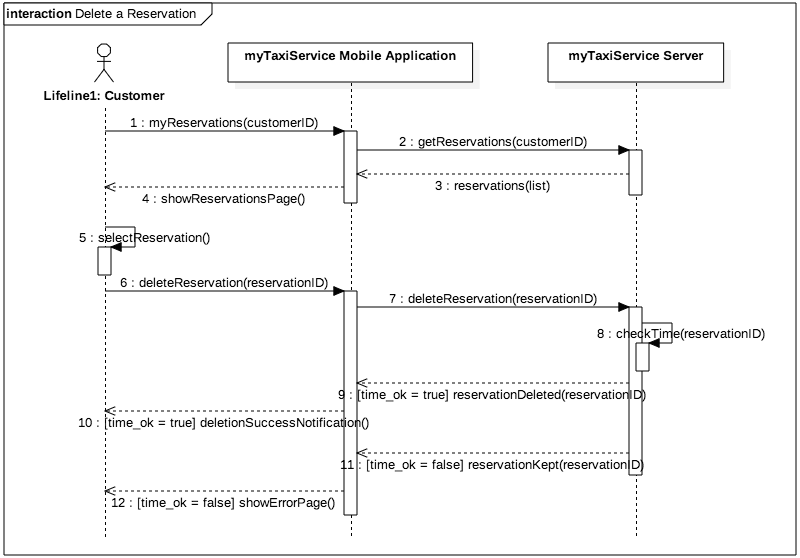
\includegraphics[width=\textwidth, scale=0.5]{IMG/InteractionDiagrams/ReservationDeletion.png}
					\caption{Reservation Deletion Interaction Diagram}\label{sec:FigureReservationDeletion}
				\end{figure}